\chapter{User Manual}

This chapter outlines how to use the developed system, both in terms of using it as it is intended as a client, as well as how to deploy the system on ones own server for testing using Docker.

\section{Client Manual}

Usage of the system is simple for the client. There are two endpoints of direct interest for the client, both on the main controller. To put it simply, there are only two web addresses that the client needs to worry about, everything else is handled behind-the-scenes. Given, for instance, the website domain "https://federicoshytte.dk/"\footnote{The service is expected to be deployed on this domain up to and during the project exam, and may be used freely. If it is for some reason down, please contact the team to request a reboot.}, the only addresses the client needs to worry about are:

\begin{itemize}
    \item https://federicoshytte.dk/room
    \item https://federicoshytte.dk/room/:roomId
\end{itemize}

The first one requests a new room to be created. The second one requests a specific room denoted by the :roomId part of the URL, usually one the client has been linked to by another person. Requesting a new room automatically redirects the client to the new room, and the room URL can then be copied from the web browsers address bar to send to others. A specific room URL might look something like this:

https://federicoshytte.dk/room/64f869a5-0f2c-40fa-a31c-bc3019cf7174

Once a room has been joined, the client is greeted by a rough user interface. An example of this is visible in figure \ref{fig:coffeebreakui}

\begin{figure}[H]
    \centering
    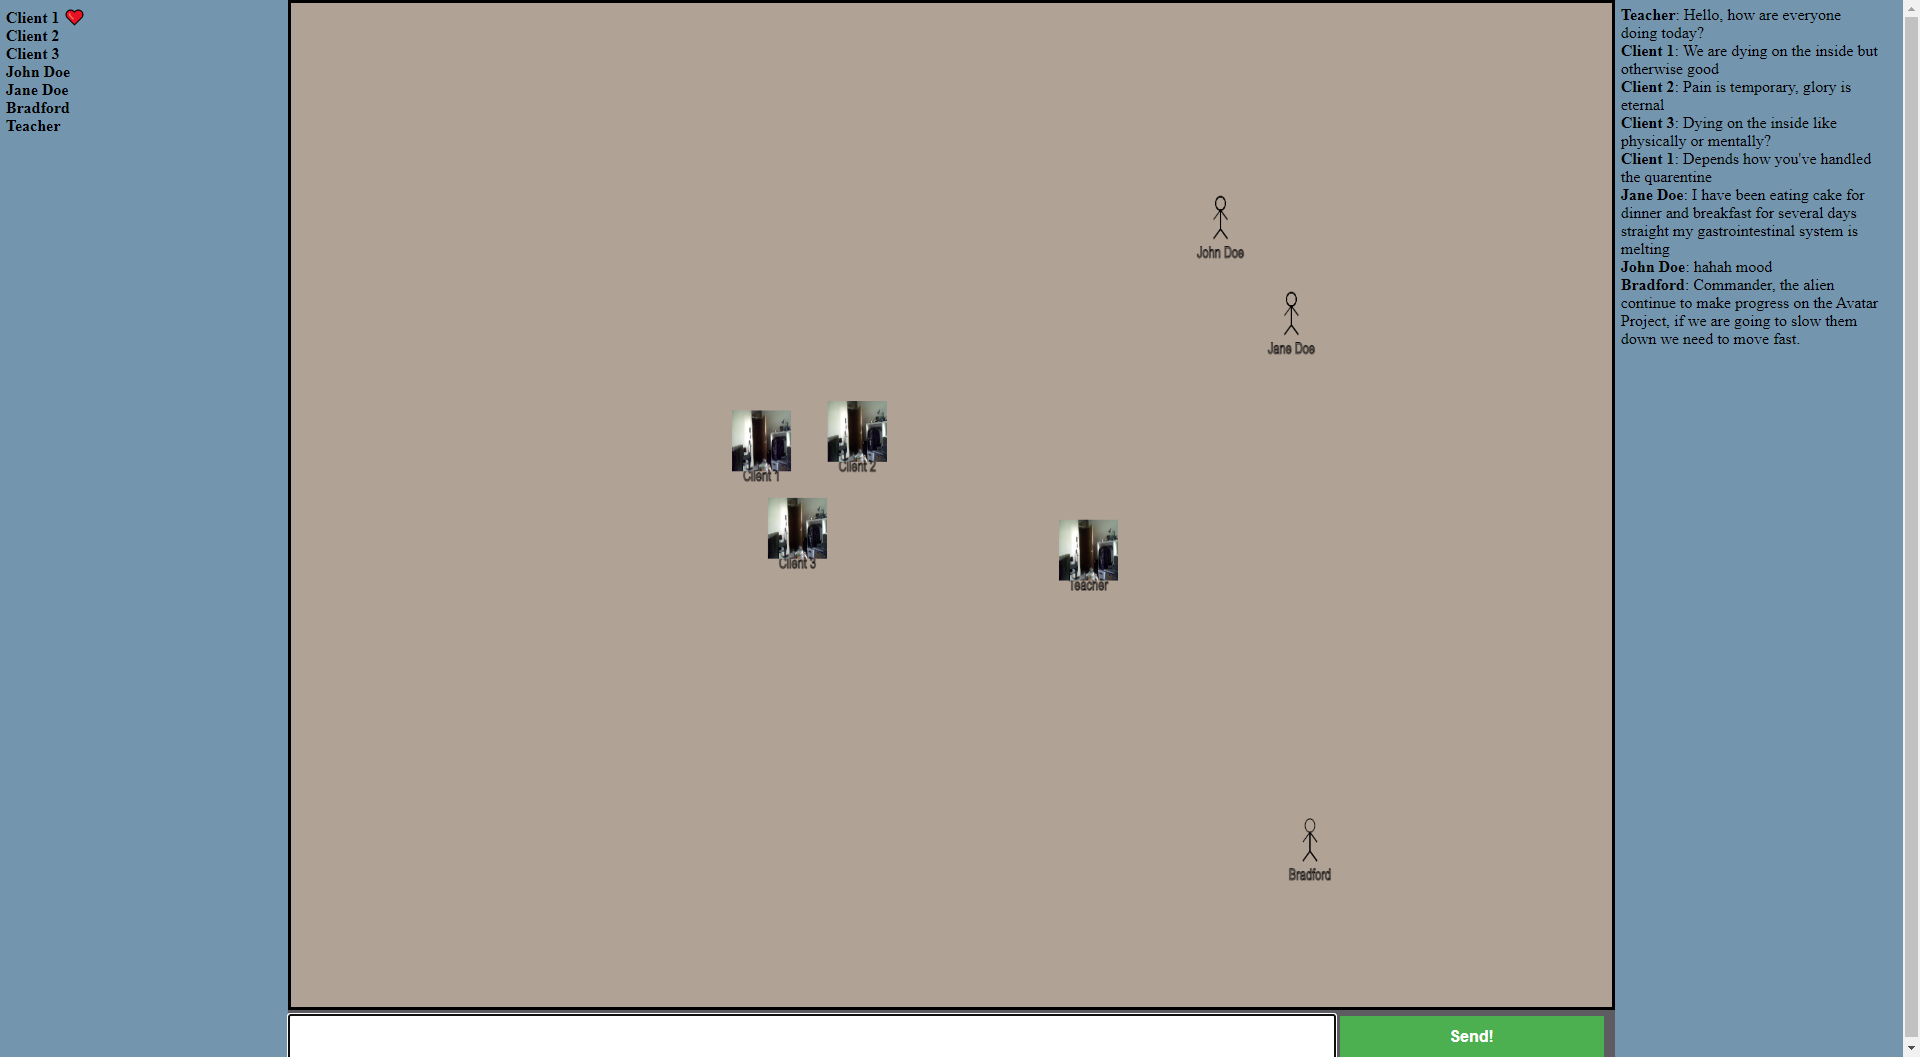
\includegraphics[width=0.75\textwidth]{Pictures/CoffeeBreakUI3.png}
    \caption{An image showing a room, with seven clients connected and spread throughout in a number of smaller groups. The picture is from the perspective Client 1, the leftmost client.}
    \label{fig:coffeebreakui}
\end{figure}

As can be seen in figure \ref{fig:coffeebreakui}, the user interface is split in three major parts. A list of connected users to the left, the virtual room rendered in the middle with a input box for chat message in the button, and finally a list of chat messages to the right. The client can move around in the room by clicking the virtual room at their desired position. Once moved, they will connect and disconnect video and voice connections to other users as they have moved in and out of an arbitrary range. These connections are shown in the figure as nearby identical webcam streams, as the picture was taken with all clients on the same physical machine.

\section{Deployment Manual}

In the GitHub repository, a docker-compose file is included. Starting this will setup a local testing environment to experiment with the system. This will be the case for both of the implemented solutions described in the report.

Docker compose deployment containing all repos requires as submodules for the two solutions are linked bellow

The P2P solution

\href{https://github.com/CoffeeBreak-Architecture/Docker-Deployment-P2P}{https://github.com/CoffeeBreak-Architecture/Docker-Deployment-P2P}

The MRS solution

\href{https://github.com/CoffeeBreak-Architecture/Docker-Deployment-MRS}{https://github.com/CoffeeBreak-Architecture/Docker-Deployment-MRS}

To clone the repository with all submodules use the following command in Git

\begin{lstlisting}[language=text]
git clone --recurse-submodules -j8 "Solution git link"
\end{lstlisting}

Afterwards just docker-compose up to start the deployment. 

If a "no build" deployment is wanted instead, go to the link below. This repository contains docker-compose files building the system out of Docker Hub images, eliminating the need to build the containers yourself.

\href{https://github.com/CoffeeBreak-Architecture/Docker-Compose-Files-Build-Free}{https://github.com/CoffeeBreak-Architecture/Docker-Compose-Files-Build-Free}


